 \subsection{Synfuels (Sebastian)}

 
 \begin{xtabular}{|p{3.8cm}|p{8.3cm}|p{4.2cm}|}
 	\vspace*{-1.25\baselineskip}\subsubsection{Topic Title}
 	& 
 	Synthetic fuels are becoming more relevant in recent times, due to the current development of the earth’s climate. 
 	& 
 	\\
 	%heading
 	
 	&
 	%main
 	To counteract this, the German government decided to eliminate pollutant emissions by 2050. One option is to use more electro mobility, but the current infrastructure isn't nearly sufficient to reach this goal. Therefore, the use of synthetic fuels might be an alternative.
 	&
 	%ref
 	\mydef{counteract - to work against something}
 	
 	\url{https://www.maierkorduletsch.de/ome-kraftstoffe-diesel-verbrennungsmotor/}
 	\\
 	\vspace*{-1.25\baselineskip}\subsubsection{Criteria}
 	& 
 	To be considered an alternative for conventional fuels, synthetic fuels must comply with some criteria. First, the fuels need to have less pollutant emissions than conventional fuels. Another criterion is, that the production cost of synthetic fuels should be either equal or less than those of conventional fuel. If the costs are higher, no one will buy the new fuel, because higher production costs lead to higher prices at gas stations.
 	&
 	\mydef{complied - act in accordance with a wish or command}
 	\\
 	\vspace*{-1.25\baselineskip}\subsubsection{Findings}
 	& 
 	All synthesis fuels use nearly the same production methods. Synthesis gas is needed, which can be obtained in different ways. This synthesis gas is then directed into a reactor, where it reacts with a catalysator to the desired fuel or substance. There are different types of synthetic fuel:
 	&
 	\mydef{obtained - get something}
 	\\
 	%heading
 	CTL fuel
 	&
 	%main
 	CTL fuels (coal-to-liquid fuels) are produced using the Bergius process. In this process coal is used as a reactant. The coal is then hydrogenated at high temperatures and pressures to form a synthetic fuel.
 	&
 	%ref
 	\url{https://de.wikipedia.org/wiki/Synthetischer_Kraftstoff}
 	\\
 	%heading
 	GTL fuel
 	&
 	%main
 	GTL fuels (gas-to-liquid fuels) use natural gas as a reactant. In the Fischer-Tropsch process the natural gas is partially oxidized to get synthesis gas. The synthesis gas is then reacting over a catalyst to produce long-chain hydrocarbons. 
 	&
 	%ref
 	\url{https://en.wikipedia.org/wiki/Gas_to_liquids}
 	\\
 	%heading
 	DME
 	&
 	%main
 	One possible GTL fuel is Dimethyl Ether (DME). The first step to produce DME is that methanol is gained from synthesis gas. In the second step methanol is dehydrated to DME.
 	&
 	%ref
 	\url{https://en.wikipedia.org/wiki/Dimethyl_ether}
 	\\
 	%heading
 	PODE
 	&
 	%main
 	Another option is Polyoxymethylene Dimethyl Ether (PODE). The synthesis starts just like the one of DME by forming methanol from synthesis gas. But in the second step the methanol is oxidized to formaldehyde, which then reacts with excess methanol to PODE.
 	&
 	%ref
 	\url{https://de.wikipedia.org/wiki/Polyoxymethylendimethylether}
 	\\
 	%heading
 	BTL fuels
 	&
 	%main
 	BTL fuels (biomass-to-liquid fuels) use biogas out of biomass as a reactant. The synthesis for this fuel is exactly like the synthesis of a GTL fuel, with the one difference, that the starting material is different.
 	&
 	%ref
 	
 	\\
 	\vspace*{-1.25\baselineskip}\subsubsection{Problems encountered}
 	&
 	One of the problems that occurred during research, is that for the most synthetic fuels you need to have nonrenewable resources like coal or natural gas. If these synthetic fuels are used, pollutant emissions might be decreased but on of the nonrenewable resources of the earth is used.
 	&
 	\\
 	\vspace*{-1.25\baselineskip}\subsubsection{Solutions}
 	& 
 	Even though CTL fuels could be a cheaper alternative for conventional fuels, because coal is cheaper, than oil. But it's carbon dioxide emissions are higher, than the emissions from conventional fuel and as already mentioned above, coal is a nonrenewable resource and therefore, for the distant future CTL fuel isn't an option.
 	&
 	\\
 	%heading
 	
 	&
 	%main
 	GTL fuels have the positive effect, that due to their chemical composition, they produce no sulfur- or nitrogen compounds and emit less carbon dioxide upon combustion. The production cost for GTL fuel are still higher, than those of conventional fuel, because there are not as much companies that produce this type of fuel and it's also not an option for the distant future, because natural gas is used as a reactant.
 	&
 	%ref
 	
 	\\
 	%heading
 	
 	&
 	%main
 	BTL fuels have the same positive effect as the GTL fuels, because the synthesis route is the same. And the disadvantages of the higher cost at gas stations are also the same. But another positive effect of BTL fuels, is that the starting material is renewable and therefore, it's an option for the distant future. 
 	&
 	%ref
 	
 	\\
 	\vspace*{-1.25\baselineskip}\subsubsection{Current Developments}
 	& 
 	At the moment, there are many companies, that do research on this topic. One of those is the Karlsruher Institute for Technology (KIT), which is working on the production of DME using biomass as a starting material.
 	{
 		\center
 		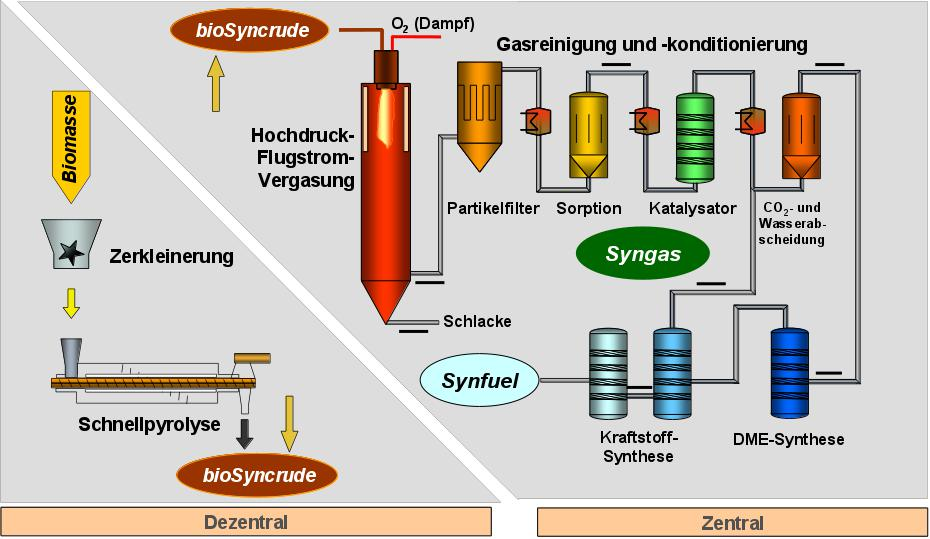
\includegraphics[width=8cm]{material/sebastian/img1.png}
 	} 
 	&
 	\url{https://www.bioliq.de/112.php}
 	\\
 	\vspace*{-1.25\baselineskip}\subsubsection{Conclusion}
 	& 
 	All these processes provide a viable alternative for conventional fuel. But considering, that the aim is to decrease the pollutant emissions and save the earth’s resources CTL fuel and GTL fuel aren't the best options. A better alternative is the production of DME or PODE with biogas. Biogas is obtained from renewable resources and therefore it's more reliable in the long term. 
 	But every option still costs more than the conventional method, which can only be changed by more research for better catalyst and more companies, which try and produce these synthetic fuels.
 	&
 	\\
 	\vspace*{-1.25\baselineskip}\subsubsection{Recommendation}
 	& 
 	At the moment, it's the best option to concentrate the development on BTL fuels like DME or PODE, because those have the biggest positive effect on the environment.
 	&
 	\\
 	\vspace*{-1.25\baselineskip}\subsubsection{Personal Comments}
 	& 
 	It was hard for me to understand how the layout should be and try to adapt my writing style to a not so academic style.
 	&
 	\\
 	\hline
 \end{xtabular}